%!TEX root = ../../thesis.tex

The \DY background is naturally split into \DYll and \DYtt processes. The former 
contributes almost exclusively to the \eech/\mmch channels,\footnote{
	In rare cases, \DYll events can enter the \emch/\mech channels. For example 
	\HepProcess{\DY \HepTo \Pmu\Pmu\Pphoton}, where a muon radiates a photon which 
	subsequently converts and is reconstructed as an electron.
}
where it is the dominant background. The latter can contribute to any channel since the 
two \HepProcess{\Ptau \HepTo \Plepton\Pnulepton\Pnut} decays are independent, though is 
doubly suppressed by the small $\text{BR}\parenths{\HepProcess{\Ptau \HepTo 
\Plepton\Pnulepton\Pnut}} = 17.6\%$ \cite{PDG:2012}.

Although \DYll does not feature prompt neutrinos, degradation of the \met resolution due 
to high pile-up can cause some \DYll events to exhibit significant \met. Since this is a 
difficult effect to model and \DYll is the dominant background to the \eech/\mmch 
channels, a high threshold of \unit{$\metrel > 40$}{\GeV} is used in the pre-selection. 
This is further tightened by tracker-based \trackmetrel cuts. On the other hand, \DYtt 
does feature prompt neutrinos and is suppressed by other cuts, such as the \mtautau veto.

The \DY backgrounds are estimated by data-driven techniques, in combination with MC 
modelling provided by \meps{\alpgen}{\fherwig}. Overlap between the \DY MC and the 
\Zgamma MC is removed through careful consideration of the MC event records.



\subsection{\DY boson transverse momentum}
\label{sec:dy:pt}

Selecting \eech/\mmch events with \unit{$\mods{\mll - \mZ} < 15$}{\GeV} results in a very 
pure sample of \DYll events, enabling the MC to be validated. In doing so, the \ptll 
distribution is found to be poorly modelled at \unit{$\ptll > 30$}{\GeV} in the 0-jet 
bin (see \Figure~\ref{fig:dy:ptZ_reweight}), despite being well modelled inclusively. 
This is unsurprising since a difficult phase space, sensitive to soft hadronic activity 
and jet shapes, has been selected: requiring a highly boosted \DY boson whilst vetoing 
events with jets. It is important to model \ptll accurately, as other observables such as 
\dphill and \ptleadlep are correlated.

For this reason, a data-driven correction to the \ptZ distribution is employed. It is 
derived in \mmch 0-jet events with \unit{$\mods{\mll - \mZ} < 15$}{\GeV}, by 
comparing the \ptll distribution observed in experimental data to that predicted by 
uncorrected MC. Each 0-jet MC event is then weighted according to its hadron-level \ptZ. 
This is found to improve the modelling of detector-level observables such as \ptll, 
\dphill and \ptleadlep (see \Figure~\ref{fig:dy:ptZ_reweight}). This correction is 
applied to the \HepProcess{\DY \HepTo \Pe\Pe/\Pmu\Pmu/\Ptau\Ptau} processes, though only 
to the 0-jet bin.

\begin{figure}[p]
	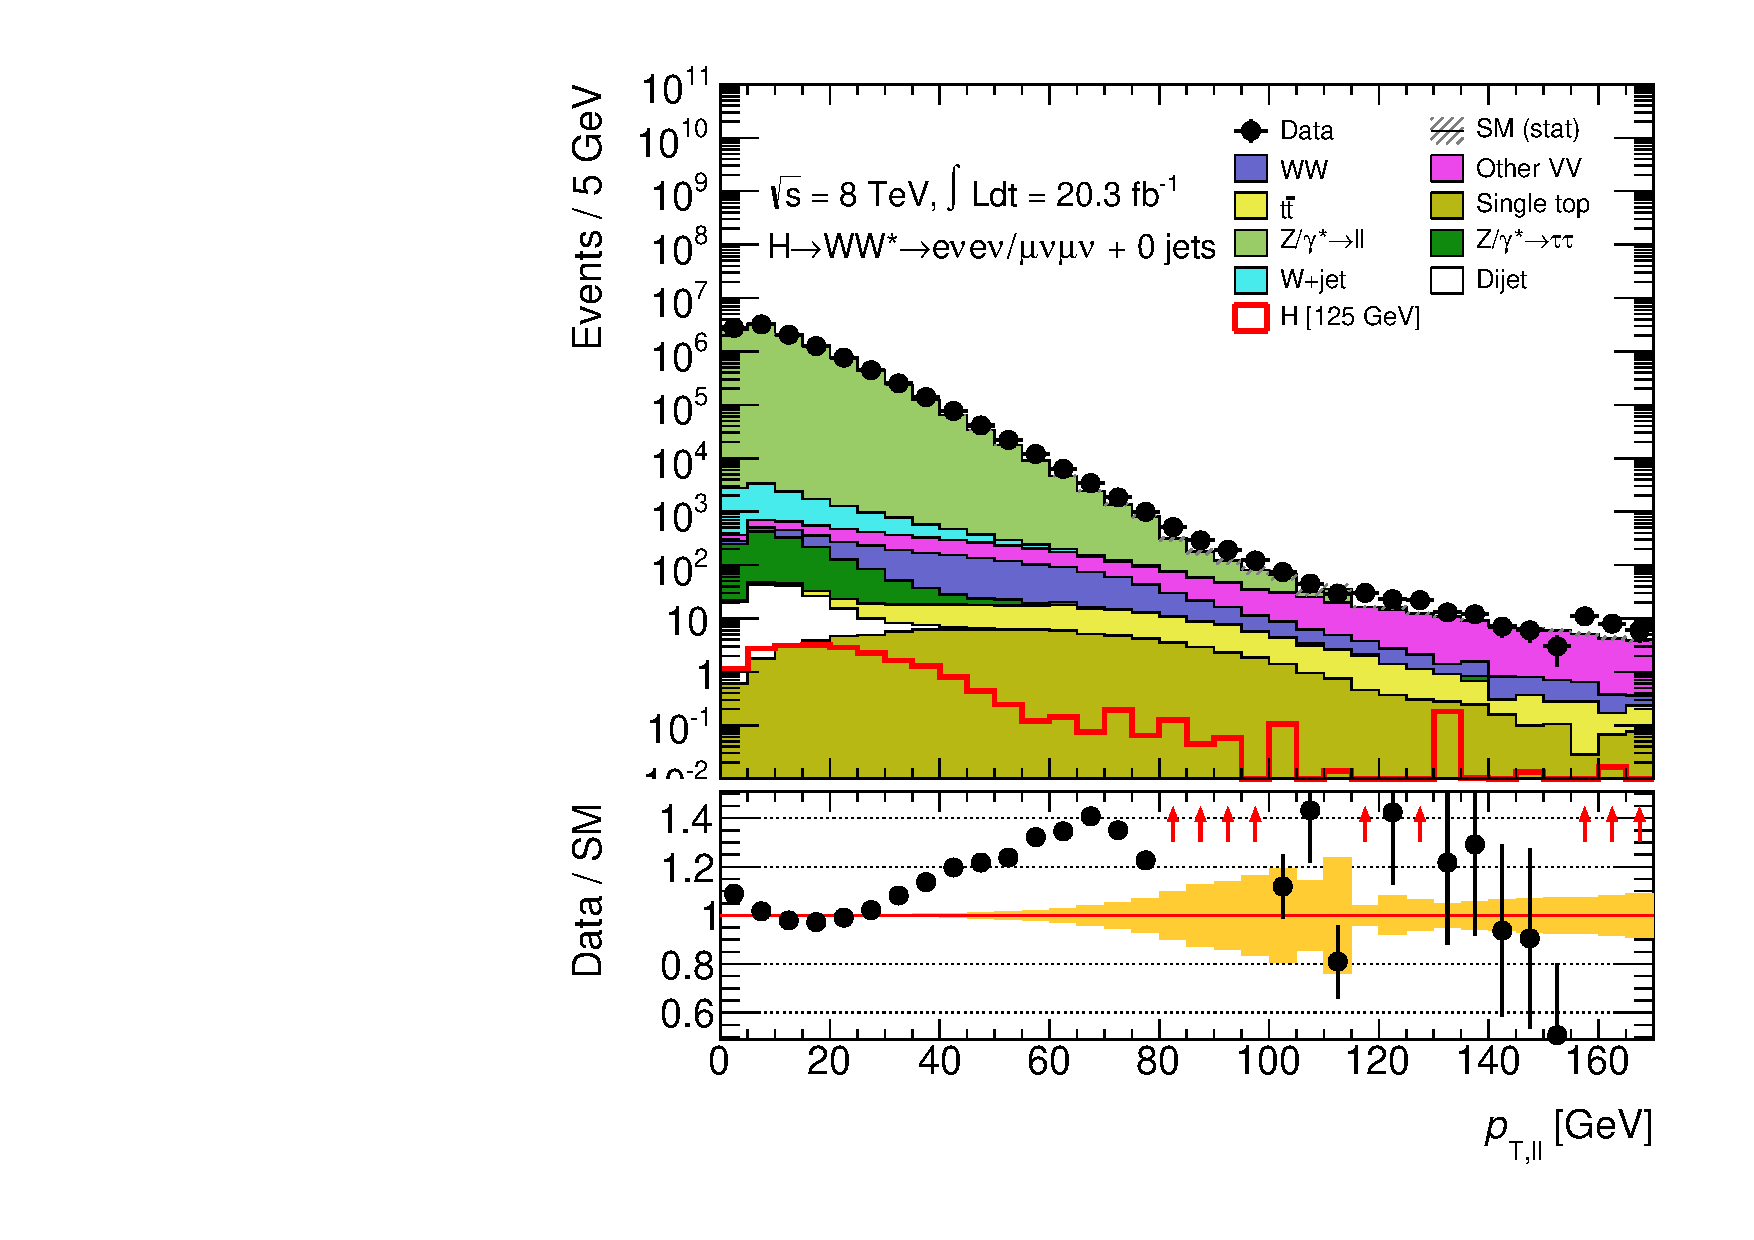
\includegraphics[width=0.48\textwidth]{tex/backgrounds/ZpT-off/eemm_CutZControl_0jet_Ptll_mh125_log}
	\hfill
	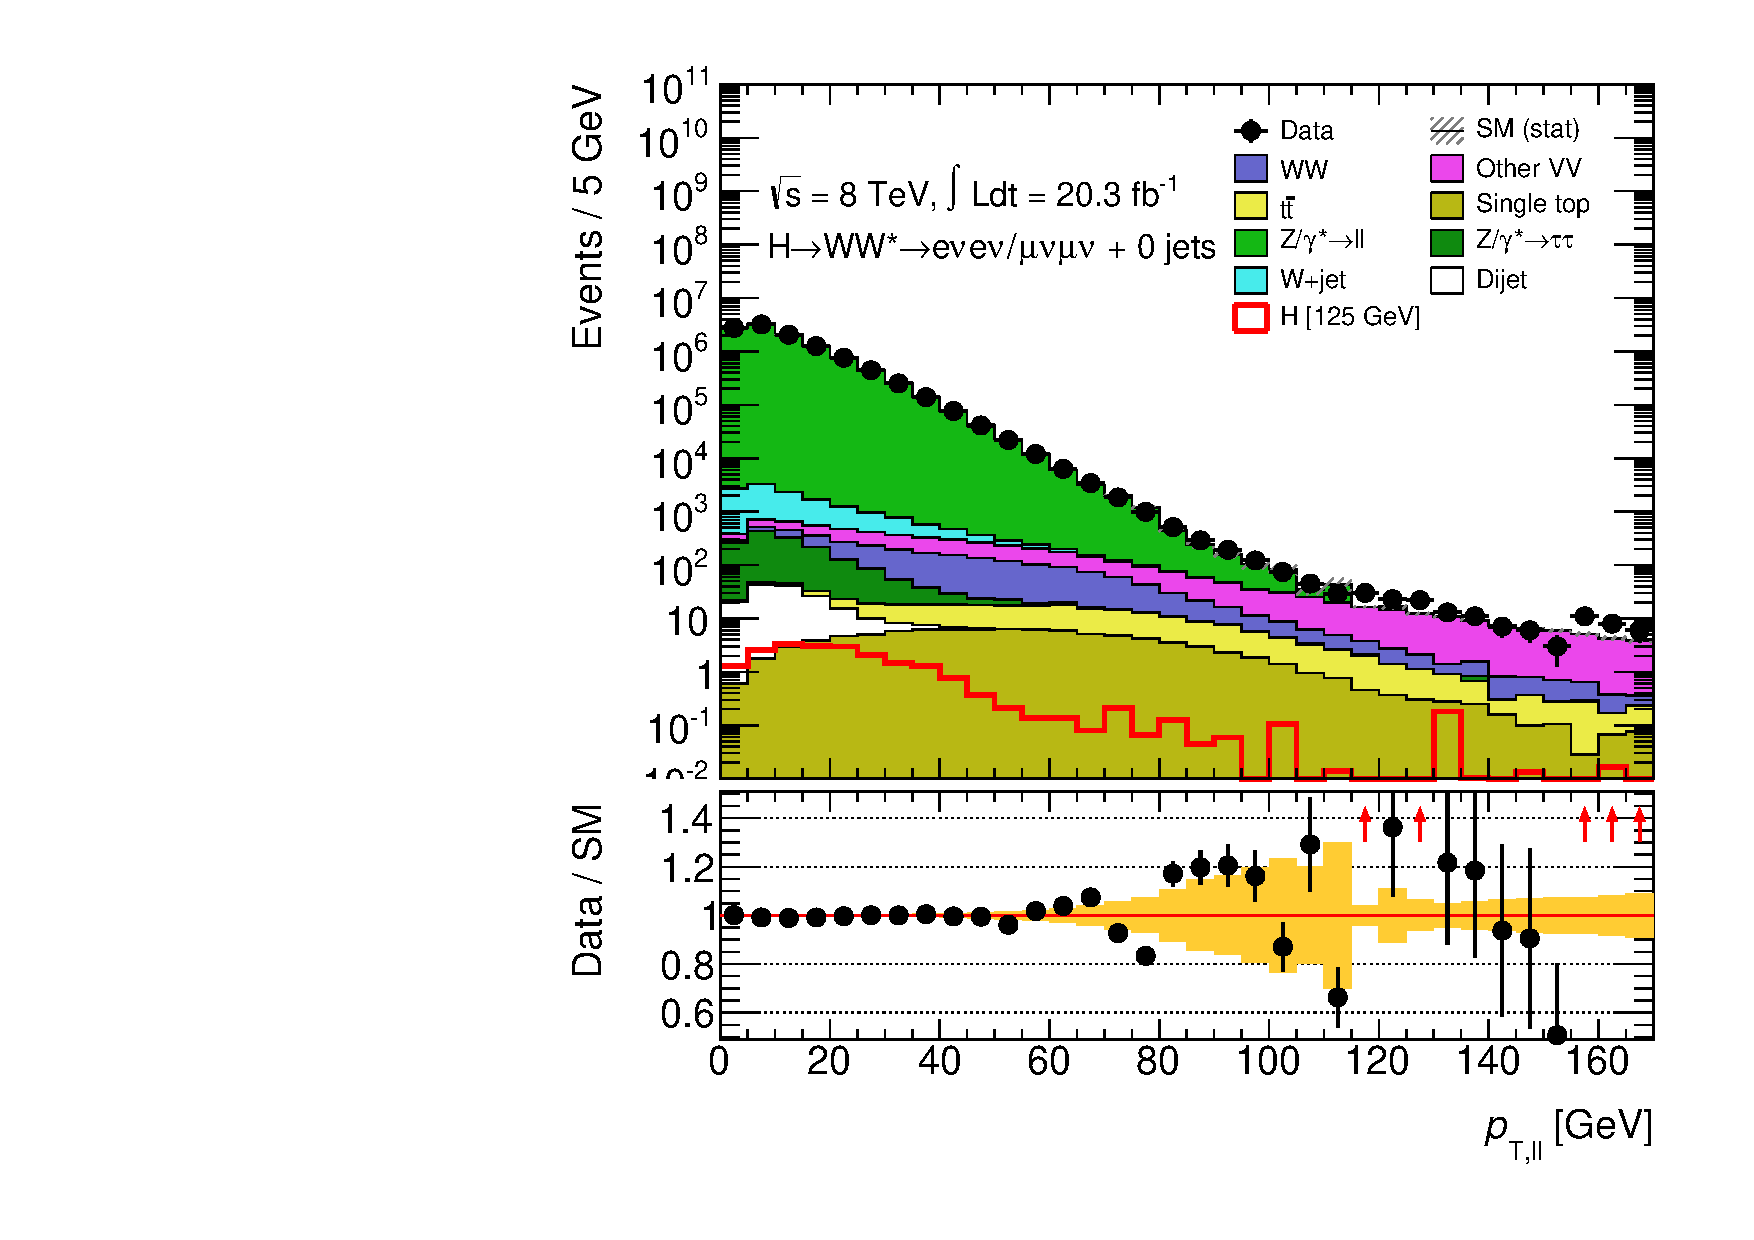
\includegraphics[width=0.48\textwidth]{tex/backgrounds/ZpT-on/eemm_CutZControl_0jet_Ptll_mh125_log}
	\\
	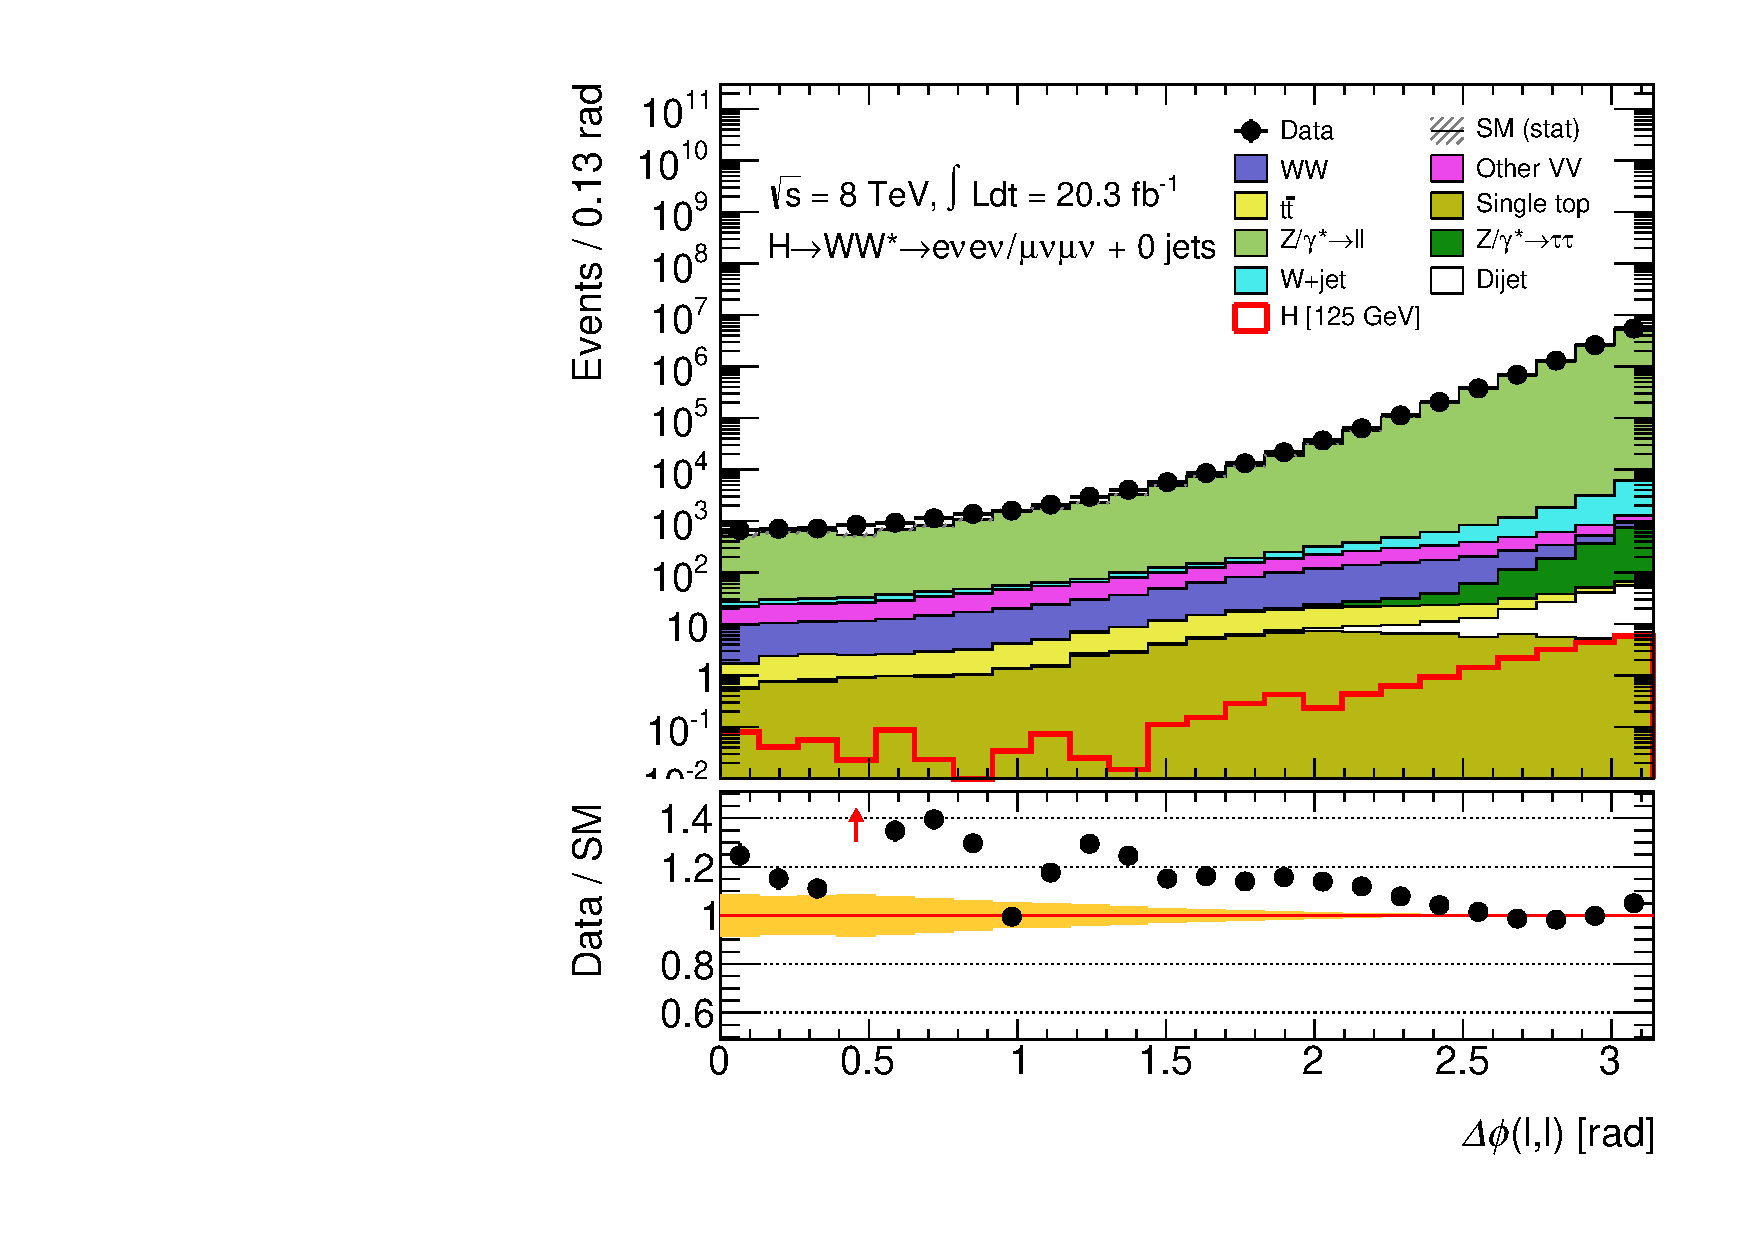
\includegraphics[width=0.48\textwidth]{tex/backgrounds/ZpT-off/eemm_CutZControl_0jet_DPhill_mh125_log}
	\hfill
	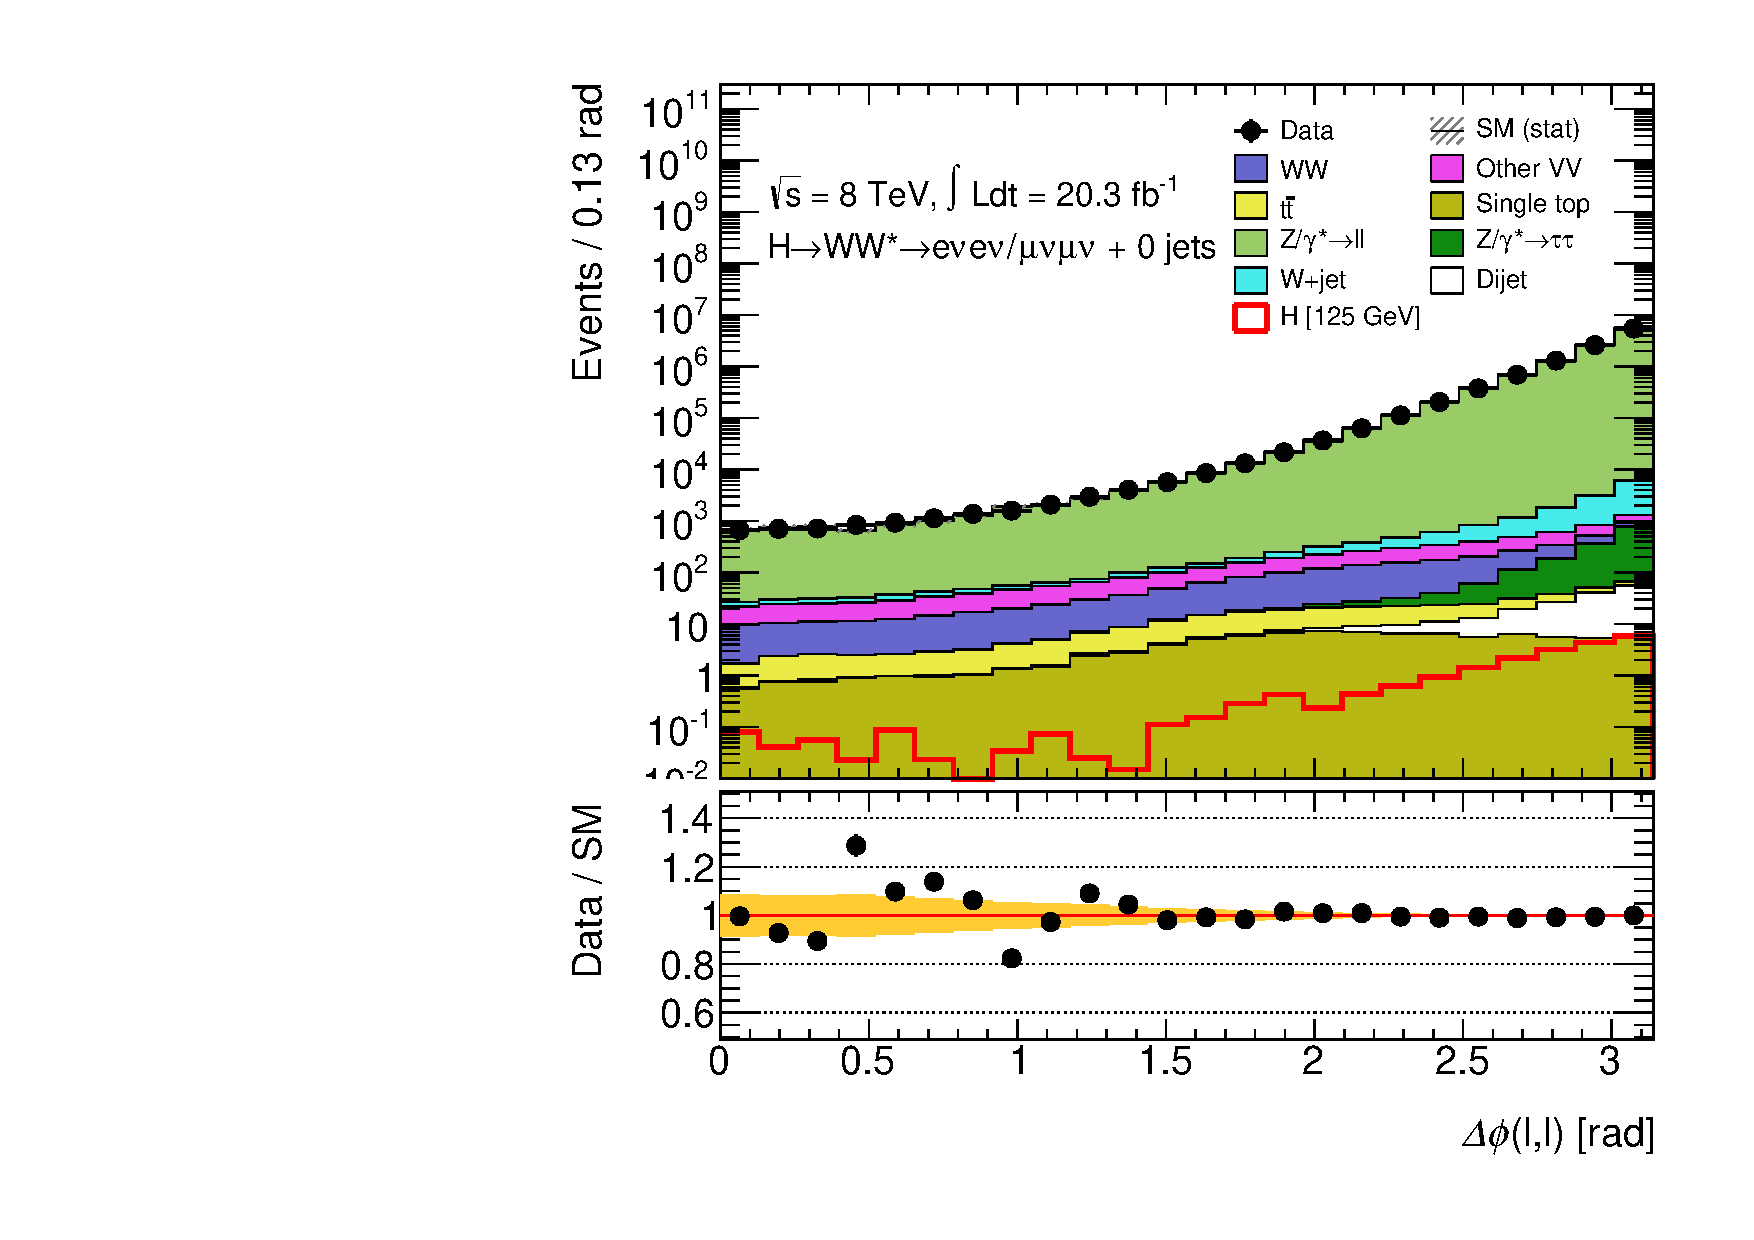
\includegraphics[width=0.48\textwidth]{tex/backgrounds/ZpT-on/eemm_CutZControl_0jet_DPhill_mh125_log}
	\\
	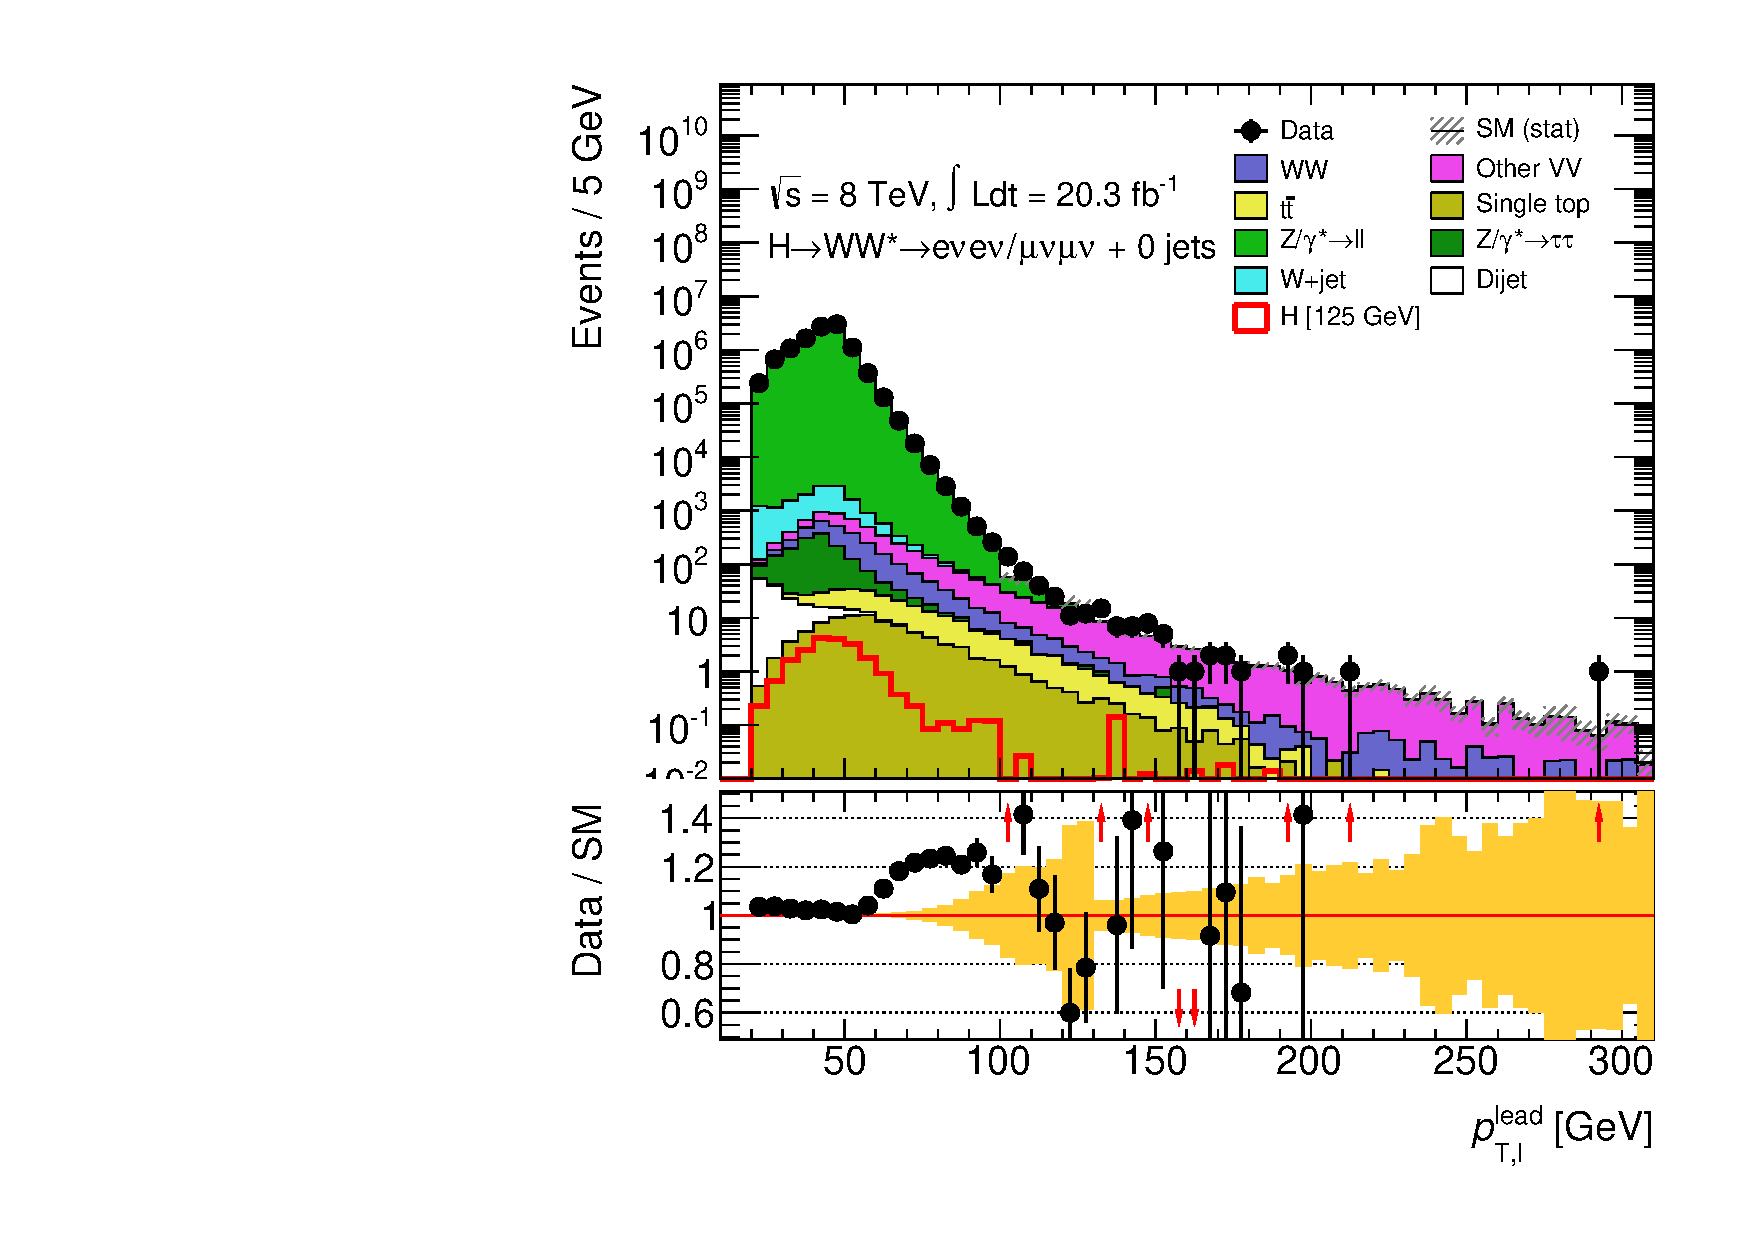
\includegraphics[width=0.48\textwidth]{tex/backgrounds/ZpT-off/eemm_CutZControl_0jet_lepPtLead_mh125_log}
	\hfill
	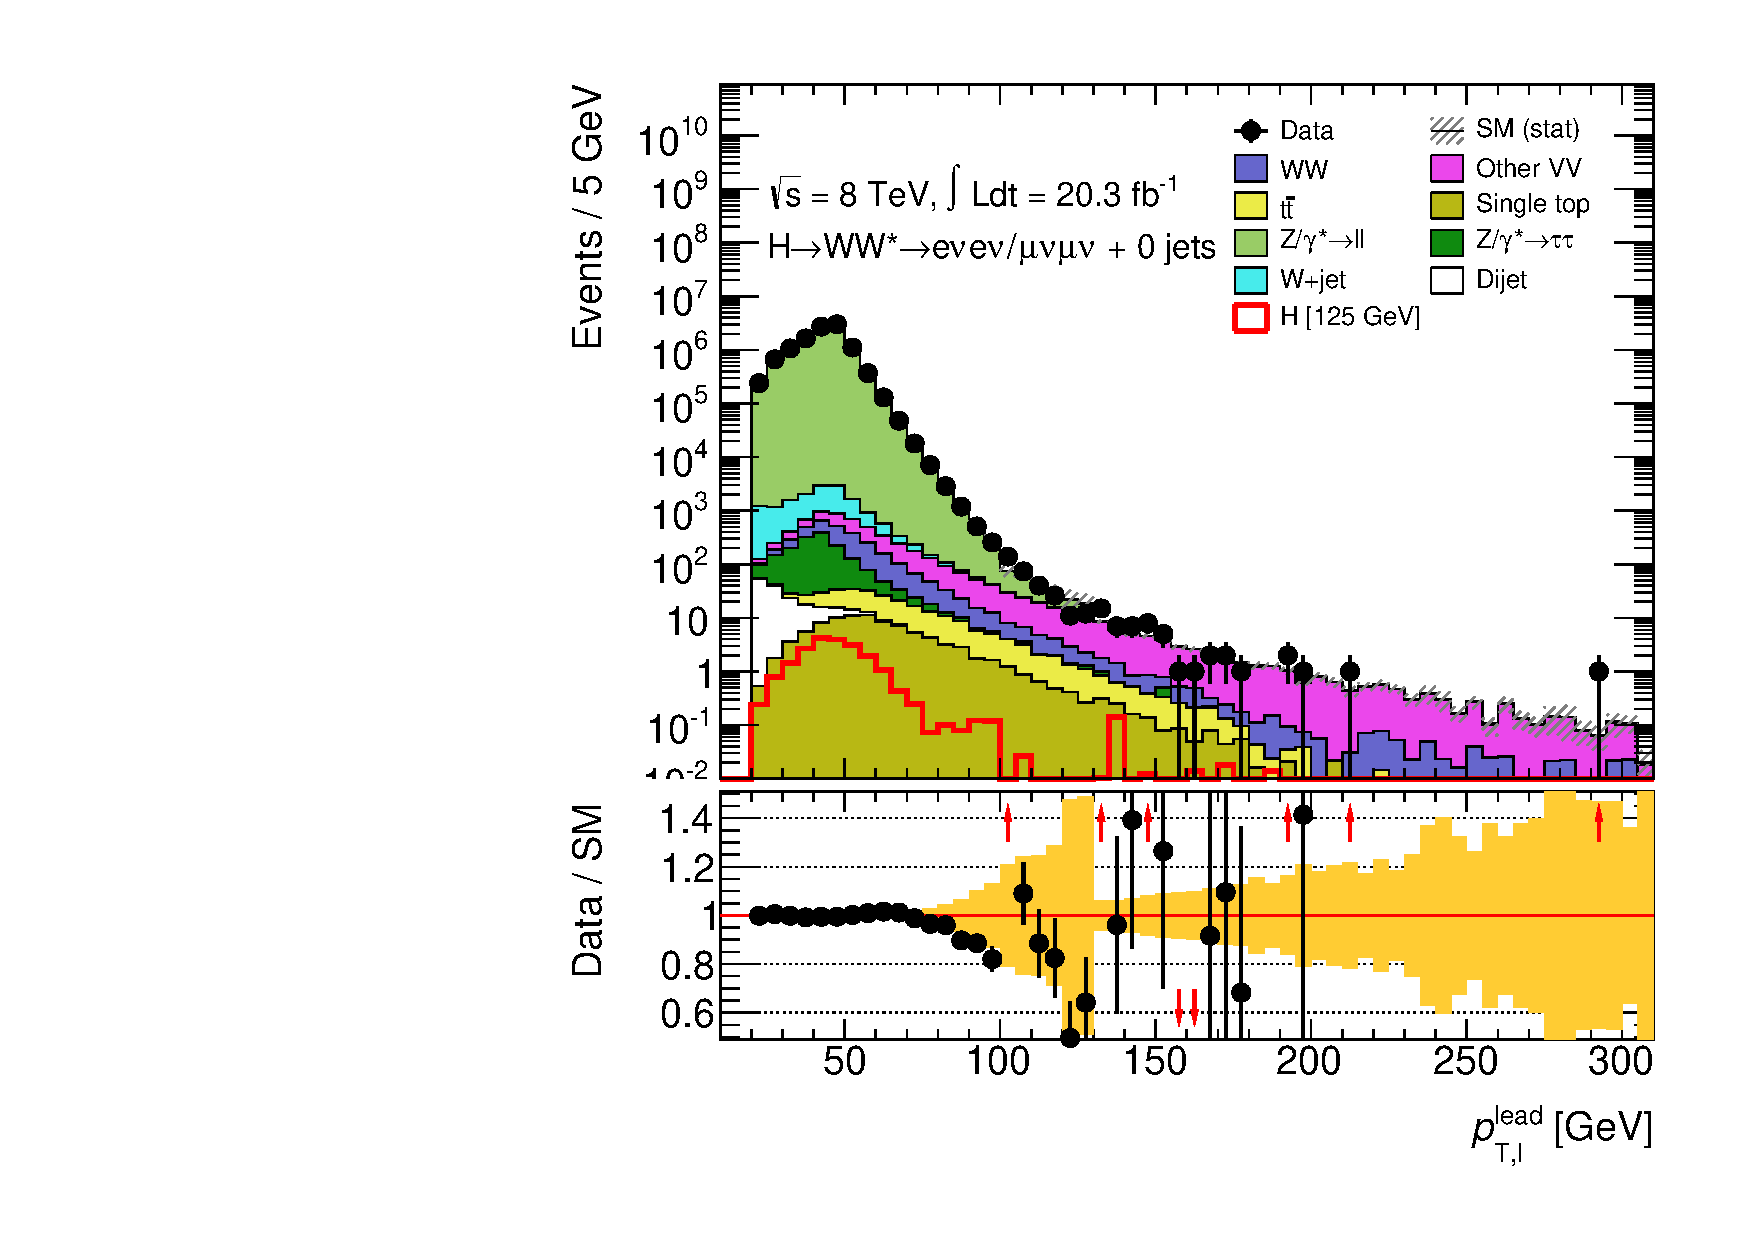
\includegraphics[width=0.48\textwidth]{tex/backgrounds/ZpT-on/eemm_CutZControl_0jet_lepPtLead_mh125_log}
	\caption{Leptonic distributions in the 0-jet \DYll control region, before (left) and 
	after (right) the \ptZ correction is applied.}
	\label{fig:dy:ptZ_reweight}
\end{figure}

The \ptZ mismodelling might be different in the signal region to the \PZ control region 
where it is derived. The validity of this extrapolation of the correction was tested by 
deriving similar corrections to \sherpa (instead of experimental data). This indicated 
there is a correlation between the correction and the \met requirement. Thus, another 
correction is derived with an additional \unit{$\corrtrackmet > 20$}{\GeV} cut, which is 
used to estimate the uncertainty in the correction.



\subsection{\DYtt estimation}
\label{sec:dy:tautau}

The \DYtt background is measured in a dedicated control region (CR), and then 
extrapolated to the signal region (SR) using MC
\begin{equation}
	N_{\HepProcess{\PZ\HepTo\Ptau\Ptau}}^{\text{pred,SR}} &= \alpha_{\HepProcess{\PZ\HepTo\Ptau\Ptau}} \cdot \parenths{N^{\text{data,CR}} - N_{\text{non-}\HepProcess{\PZ\HepTo\Ptau\Ptau}}^{\text{pred,CR}}} \\
	\alpha_{\HepProcess{\PZ\HepTo\Ptau\Ptau}} &= N_{\HepProcess{\PZ\HepTo\Ptau\Ptau}}^{\text{MC,SR}} / N_{\HepProcess{\PZ\HepTo\Ptau\Ptau}}^{\text{MC,CR}} \,.
\end{equation}
Jet-binned CRs are defined in the \emch{}+\mech channel, according to the event selection 
criteria in \Table~\ref{tab:dytt_cr_sel}. This \emch{}+\mech CR is used to extrapolate to 
each of the \emch/\mech/\eech/\mmch SRs.

\begin{table}[t]
	\begin{tabularx}{0.7\textwidth}{YYY}
		\toprule
		\multicolumn{3}{c}{\emch/\mech} \\
		\midrule
		\multicolumn{3}{c}{$\ptleadlep > 22$ and $\ptsubleadlep > 10$} \\
		\multicolumn{3}{c}{$\mll > 12$} \\
		\multicolumn{3}{c}{$\corrtrackmet > 20$} \\
		\cmidrule(lr){1-3}
		0-jet bin & 1-jet bin & \twojet bin \\
		\cmidrule(lr){1-3}
		-- & $\nbjets = 0$ & $\nbjets = 0$ \\
		-- & $\maxmtw > 50$ & -- \\
		-- & $\mtautau > \mZ - 25$ & -- \\
		-- & -- & Fail CJV or OLV \\
		$\mll < 80$ & $\mll < 80$ & $\mll < 70$ \\
		$\dphill > 2.8$ & -- & $\dphill > 2.8$ \\
		\bottomrule
	\end{tabularx}
	\caption{Event selection criteria of the \DYtt control regions. Cuts on energy, 
	momentum and mass are given in \GeV, and angular cuts are given in radians. The 
	relevant variables are described in 
	\Chapter~\ref{chap:selection}.}
	\label{tab:dytt_cr_sel}
\end{table}

\begin{figure}[t]
	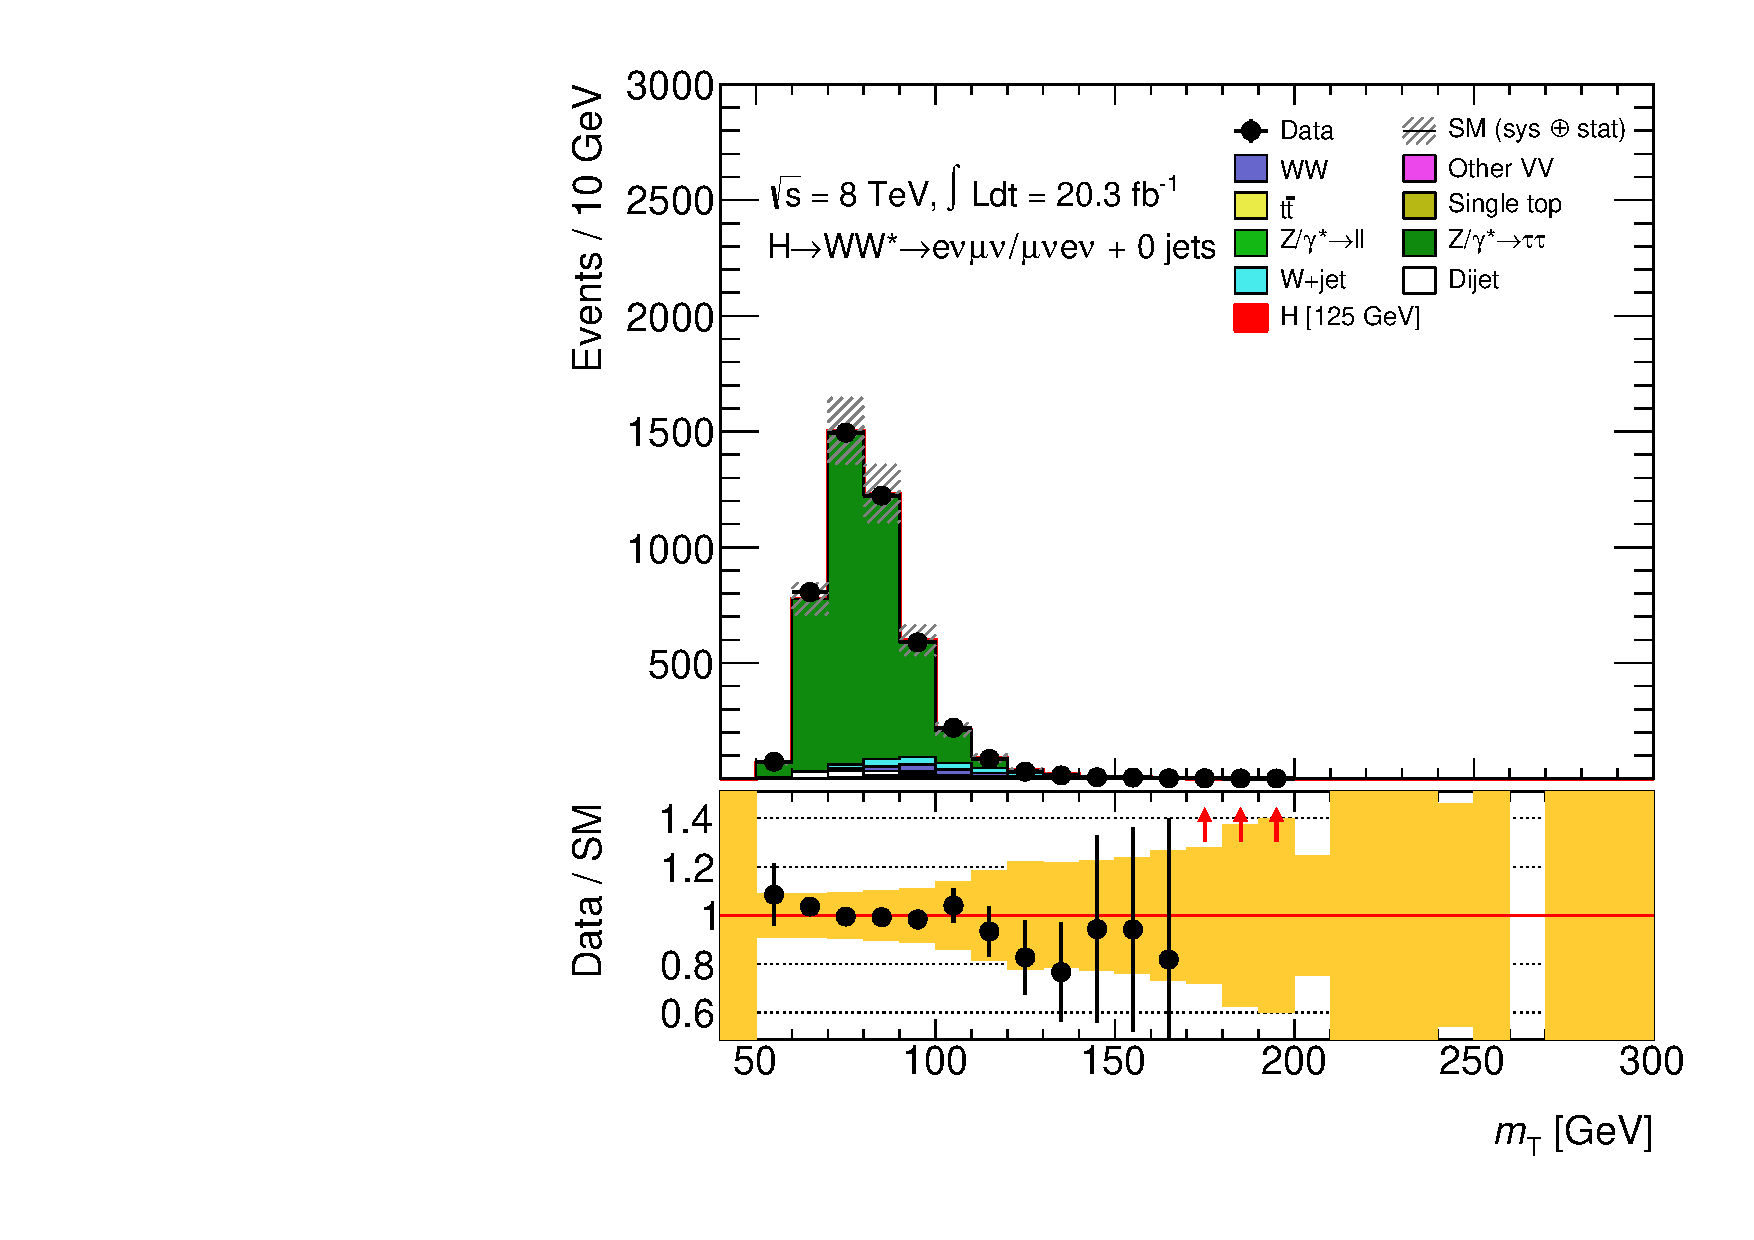
\includegraphics[width=0.495\textwidth]{tex/backgrounds/emme_CutZttControl_0jet_MT_TrackHWW_Clj_mh125_lin}
	\hfill
	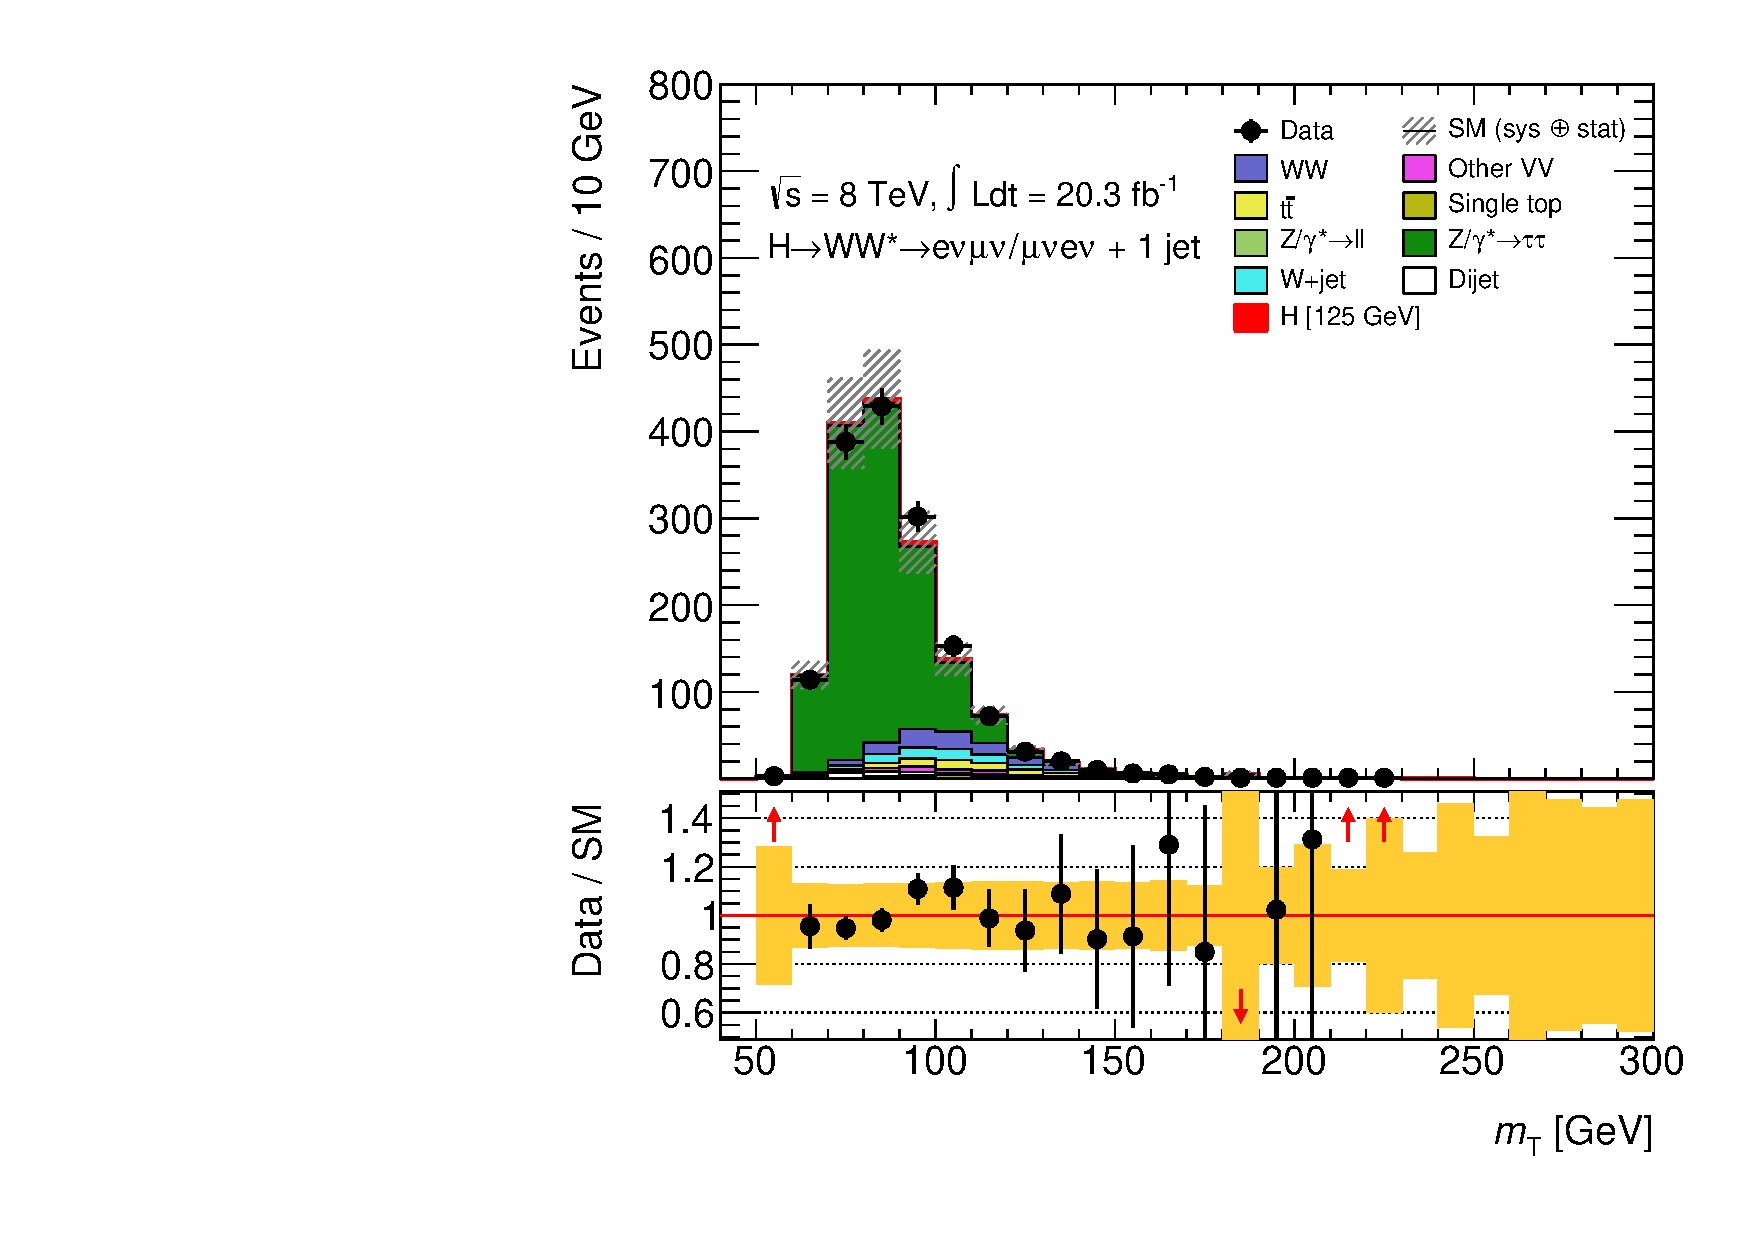
\includegraphics[width=0.495\textwidth]{tex/backgrounds/emme_CutZttControl_1jet_MT_TrackHWW_Clj_mh125_lin}
	\\
	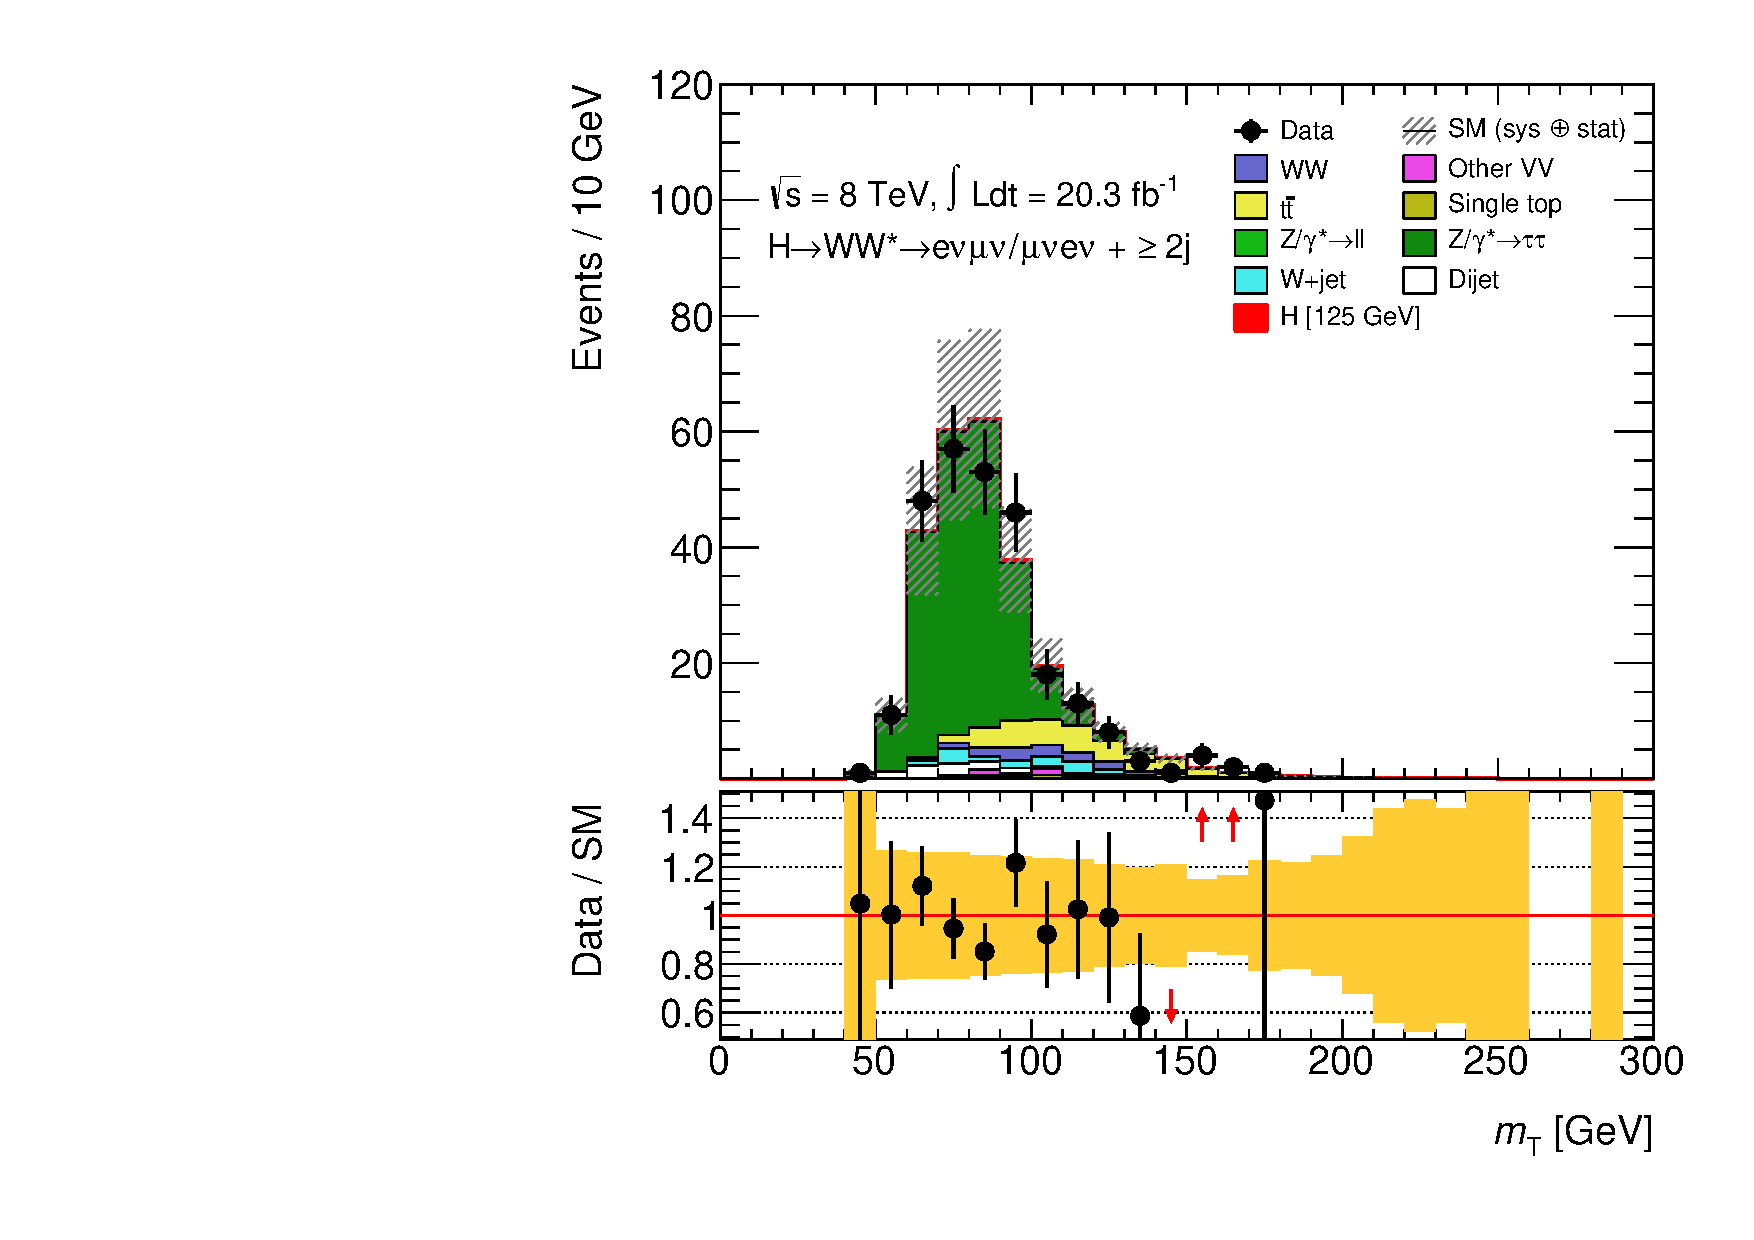
\includegraphics[width=0.495\textwidth]{tex/backgrounds/emme_CutFailVBFZttCR_2jetincl_MT_TrackHWW_Clj_mh125_lin}
	\caption{The \mt distribution in the \DYtt control regions of the 0-jet (left), 1-jet 
	(right) and \twojet (bottom) bins. Normalisation factors are applied.}
	\label{fig:dytt:cr}
\end{figure}

To estimate the \DYtt background in regions other than the SR, the method is viewed as 
providing a simple data-driven normalisation factor. This is equivalent to neglecting the 
extrapolation uncertainties, but is helpful when plotting observables. The normalisation 
factors are measured to be \stat{1.01}{0.02} in the 0-jet bin, \stat{1.08}{0.04} in the 1-jet 
bin, and \stat{1.05}{0.10} in the \twojet bin\todo{update}. \Figure~\ref{fig:dytt:cr} 
exhibits the excellent MC modelling of this background, following application of the 
normalisation factors.



\subsection{\DYll estimation}
\label{sec:dy:ll}

\DYll is the dominant background to the \eech/\mmch channels, and this section will 
describe how it is estimated in the corresponding 0-jet and 1-jet bins (the \twojet bin 
is unused in the \eech/\mmch channels).

\DYll is largely rejected by the \PZ boson mass veto, 
\unit{$\mods{\mll - \mZ} > 15$}{\GeV}, and the requirement of large missing transverse 
momentum, \unit{$\metrel > 40 (40)$}{\GeV} and \unit{$\trackmetrel > 40 (35)$}{\GeV} in 
the 0-jet (1-jet) bin. Although the \met resolution is broadened by pile-up, for 
surviving events to possess such high \metrel and \trackmetrel suggests some mismeasured 
hadronic activity recoiling against the dilepton (+ jet) system. This is also enhanced 
by the \unit{$\ptll > 30$}{\GeV} cut in the 0-jet bin.

This hadronic recoil must be soft and broad in order to avoid passing the jet 
reconstruction, and might not be modelled accurately. It is therefore preferable to use 
a data-driven estimation of this background. Fortunately, the \frecoil observable 
(described below) can discriminate \DYll from other processes in this phase space, and 
can simultaneously be used to suppress and estimate the \DYll background.

First, soft jets with \unit{$\pt > 10$}{\GeV} and $\mods{\eta} < 4.5$ are found, 
following the jet selection detailed in \Section~\ref{sec:objects:jets} minus the JVF 
cut. In the 0-jet bin, \frecoil is defined by
\begin{equation}
	\frecoil = \left. \mods{\sum\limits_{j\text{ in }\wedge} \text{JVF}_{j} \cdot \bvec{p}_{\text{T,}j}} \, \middle/ \ptll \right.
	\label{eq:dy:frecoil}
\end{equation}
where $\wedge$ is the detector quadrant centred on $-\ptllvec$. This is the fraction of 
\ptll that can be balanced by soft hadronic activity in the opposing quadrant. 
In the 1-jet bin, it is the dilepton + jet system that must be balanced, and thus the 
quadrant $\wedge$ is centred upon $-\ptlljvec$ and the denominator becomes \ptllj.

The tight \met criteria sculpt \frecoil in \DYll towards higher values, whereas the other 
background processes (and signal) feature high-\pt neutrinos and peak at lower values 
(see \Figure~\ref{fig:dy:frecoil_shape}). A \textit{template method} exploits the 
markedly different \frecoil shape of the \DYll background to estimate its contribution to 
the \eech/\mmch signal regions.

\begin{figure}[t]
	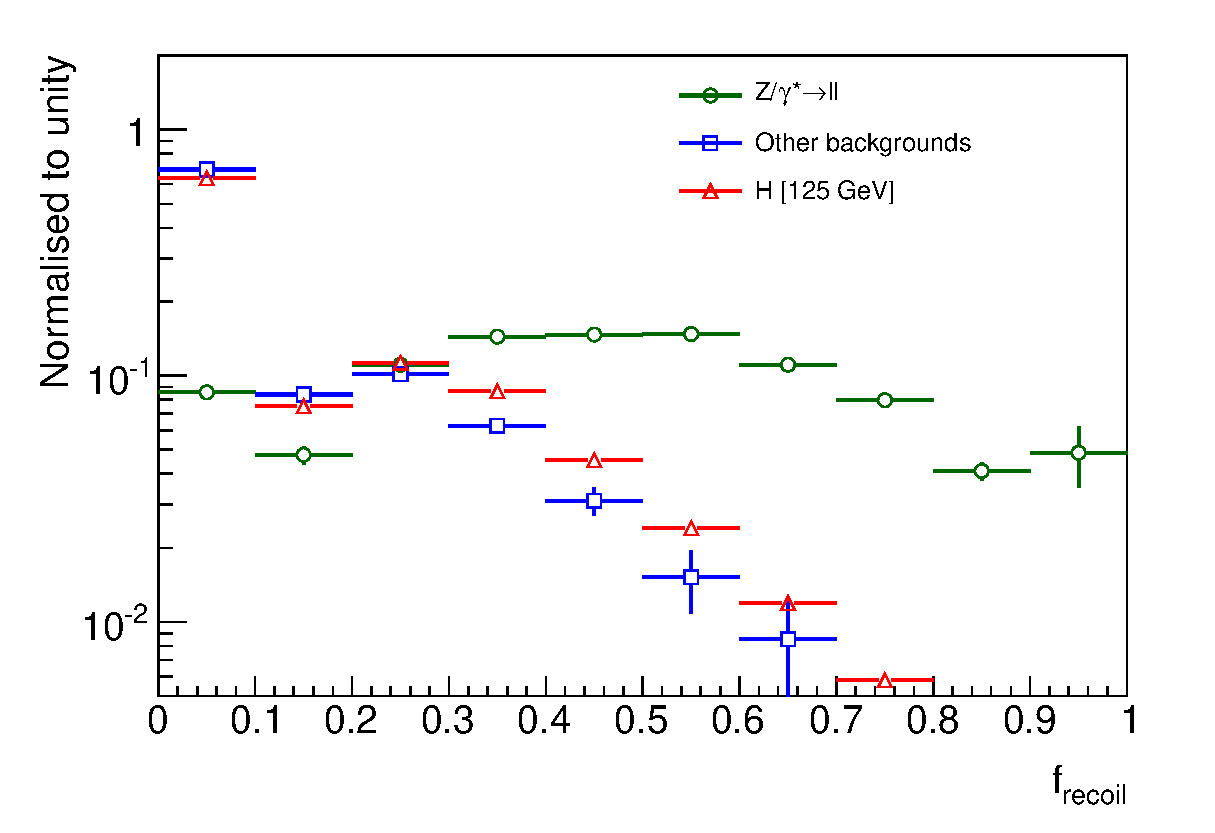
\includegraphics[width=0.495\textwidth]{tex/backgrounds/frecoil_0jet}
	\hfill
	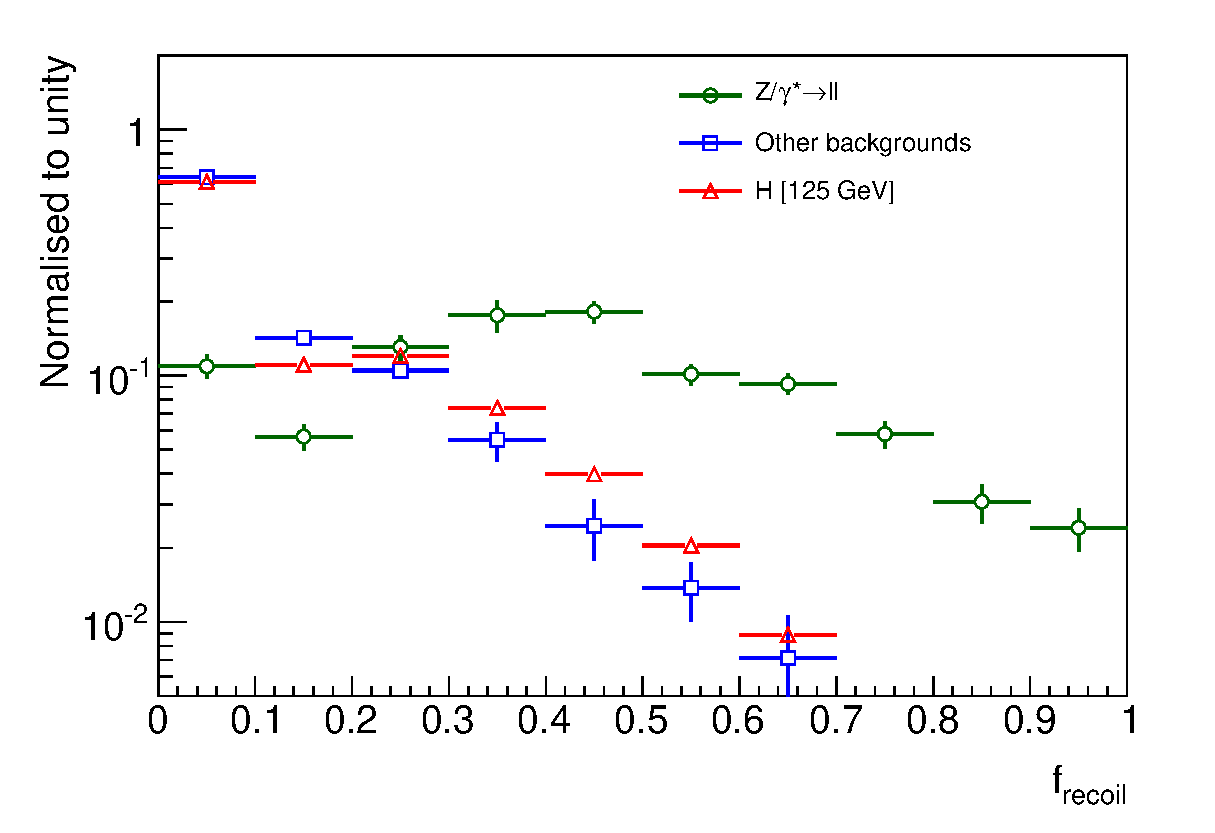
\includegraphics[width=0.495\textwidth]{tex/backgrounds/frecoil_1jet}
	\caption{\frecoil shape in the 0-jet (left) and 1-jet (right) signal regions of the 
	\eech/\mmch channels, excluding the \frecoil cut itself. The other backgrounds 
	are modelled by data-driven methods described elsewhere, while the \DYll and signal 
	processes are described by MC.}
	\label{fig:dy:frecoil_shape}
\end{figure}

In the template method, the signal region (SR) is defined by the full event selection of 
the \eech/\mmch channels, excluding the \frecoil cut (whose efficiency shall be predicted 
by the method). The \frecoil distribution $\mathcal{T}$ in the SR of the same-flavour 
(SF) channels, \ie the \eech/\mmch channels, has two components with distinct shapes: 
\DYll and other processes (including signal). If the shape of both components are 
predicted, then their relative contributions can be fit using the observed \frecoil 
distribution in the SR
\begin{equation}
	\mathcal{T}^{\text{data,SR,SF}} = K^{\text{fit}}_{\text{non-}\HepProcess{\PZ\HepTo\Plepton\Plepton}} \cdot \mathcal{T}^{\text{pred,SR,SF}}_{\text{non-}\HepProcess{\PZ\HepTo\Plepton\Plepton}} + K^{\text{fit}}_{\HepProcess{\PZ\HepTo\Plepton\Plepton}} \cdot \mathcal{T}^{\text{pred,SR,SF}}_{\HepProcess{\PZ\HepTo\Plepton\Plepton}}
	\label{eq:dy:pacman_basic}
\end{equation}
where $K^{\text{fit}}_{i}$ are prefactors determined by the fitting procedure, and the 
input distributions $\mathcal{T}^{\text{pred,SR,SF}}_{i}$ are determined by data-driven 
methods described below.

$\mathcal{T}^{\text{pred,SR,SF}}_{\text{non-}\HepProcess{\PZ\HepTo\Plepton\Plepton}}$ 
is determined from the observed distribution in different-flavour (DF) events, \ie the 
\emch/\mech channels, $\mathcal{T}^{\text{data,SR,DF}}$. Note that this DF distribution 
is measured in the SR defined by SF event selection criteria. In doing this, the 
normalisation factor $K^{\text{fit}}_{\text{non-}\HepProcess{\PZ\HepTo\Plepton\Plepton}}$ 
becomes an extrapolation parameter 
$\alpha_{\text{non-}\HepProcess{\PZ\HepTo\Plepton\Plepton}}^{\text{fit}}$ from DF to SF. 
This method is valid because the \DYll background to the SF channels is negligible, and 
the composition of the other processes is consistent between DF and SF events.

$\mathcal{T}^{\text{pred,SR,SF}}_{\HepProcess{\PZ\HepTo\Plepton\Plepton}}$ is determined 
from the SF distribution measured in a \DYll control region (CR) 
$\mathcal{T}^{\text{data,SR,DF}}$. The CR is defined by the same selection criteria as 
the SR, except that the \unit{$\mll < 55$}{\GeV} criteria becomes 
\unit{$\mods{\mll - \mZ} < 15$}{\GeV}. As the \met and \ptll criteria remain in the CR 
definition, \frecoil is sculpted similarly to the SR. However, this also means that the 
contribution of other processes in the CR is non-negligible and must be subtracted. This 
contamination is estimated from the distribution measured in DF events passing the same 
CR selection $\mathcal{T}^{\text{data,CR,DF}}$, with the extrapolation from DF to SF 
predicted by dedicated data-driven methods described elsewhere or by MC.

Thus, (\ref{eq:dy:pacman_basic}) becomes
\begin{equation}
	\mathcal{T}^{\text{data,SR,SF}} = \alpha_{\text{non-}\HepProcess{\PZ\HepTo\Plepton\Plepton}}^{\text{fit}} \cdot \mathcal{T}^{\text{data,SR,DF}} + \alpha_{\HepProcess{\PZ\HepTo\Plepton\Plepton}}^{\text{fit}} \cdot \parenths{\mathcal{T}^{\text{data,CR,SF}} - \alpha_{\text{non-}\HepProcess{\PZ\HepTo\Plepton\Plepton}}^{\text{pred}} \cdot \mathcal{T}^{\text{data,CR,DF}}}
	\label{eq:dy:pacman_full}
\end{equation}
where $\alpha_{\text{non-}\HepProcess{\PZ\HepTo\Plepton\Plepton}}^{\text{fit}}$ and 
$\alpha_{\text{non-}\HepProcess{\PZ\HepTo\Plepton\Plepton}}^{\text{pred}}$ are 
extrapolations from DF to SF, and 
$\alpha_{\HepProcess{\PZ\HepTo\Plepton\Plepton}}^{\text{fit}}$ is an extrapolation in 
\mll. Note that the $\alpha_i$ are prefactors and leave template shapes unchanged. The 
sensitivity of this method to the signal strength is tested and found to be negligible. 

The final event selection criterion in the \eech/\mmch channels is $\frecoil < 0.1$. The 
efficiency of this cut for both \DYll and other processes is inherently predicted by the 
template method. To simplify matters, the templates are reduced to two bins: 
$\frecoil < 0.1$ and $\frecoil > 0.1$. With two bins and two free parameters 
$\alpha^{\text{fit}}_i$, the system can be solved exactly. The dominant uncertainty in 
the 0-jet \DYll estimation arises from correlations between \frecoil and \mll, and is 
evaluated with MC to be 32\%. The 1-jet bin is dominated by statistical uncertainties.

